\documentclass{article}

\title{Algorytmy Tekstowe\\Trie i drzewa sufiksów - raport}
\author{Jakub Pinowski}
\date{}

\usepackage{graphicx}
\begin{document}
	\maketitle
	Do testów użyte zostało pięć przykładowych tekstów:
	\begin{itemize}
    \item bbb\$
    \item aabbabd
    \item ababcd
    \item abcbccd
    \item tekst z pliku "1997\_714.txt"
	\end{itemize}
	
	\section{Porównanie czasów działania}
	\subsection{bbb\$}
		\begin{itemize}
		\item Trie: 0.0596ms
		\item Simple suffix tree building: 0.0648ms
		\item McCreight: 0.0741ms
		\end{itemize}
		
	\subsection{aabbabd}
		\begin{itemize}
		\item Trie: 0.078ms
		\item Simple suffix tree building: 0.108ms
		\item McCreight: 0.147ms
		\end{itemize}
	
	\subsection{ababcd}
		\begin{itemize}
		\item Trie: 0.0236ms
		\item Simple suffix tree building: 0.03ms
		\item McCreight: 0.0265ms
		\end{itemize}
		
	\subsection{abcbccd}
		\begin{itemize}
		\item Trie: 0.4418ms
		\item Simple suffix tree building: 0.0760ms
		\item McCreight: 0.0679ms
		\end{itemize}
		
	\subsection{Pierwsze 2000 znaków tekstu z pliku "1997\_714.txt"}
		\begin{itemize}
		\item Trie: 5.3250s
		\item Simple suffix tree building: 0.0198s
		\item McCreight: 0.007s
		\end{itemize}
		
	\subsection{Tekst z pliku "1997\_714.txt"}
		\begin{itemize}
		\item Simple suffix tree building: 3.9253s
		\item McCreight: 2.1463s
		\end{itemize}
	
	\noindent Niestety stworzenie struktury trie dla całego pliku 1997\_714.txt wymagałoby zbyt dużo pamięci jak na możliwości przeciętnego, domowego komputera, więc porównanie ograniczyło się tylko do 2000 pierwszych znaków (co i tak wymagało kilku gigabajtów miejsca) i dobitnie pokazało jak słabo wypada proste budowanie trie, nawet w porównaniu z prostym budowaniem drzewa suffiksów.   
	
	\section{Przykładowo zbudowane struktury}
	\begin{figure}[htp]
	\centering
	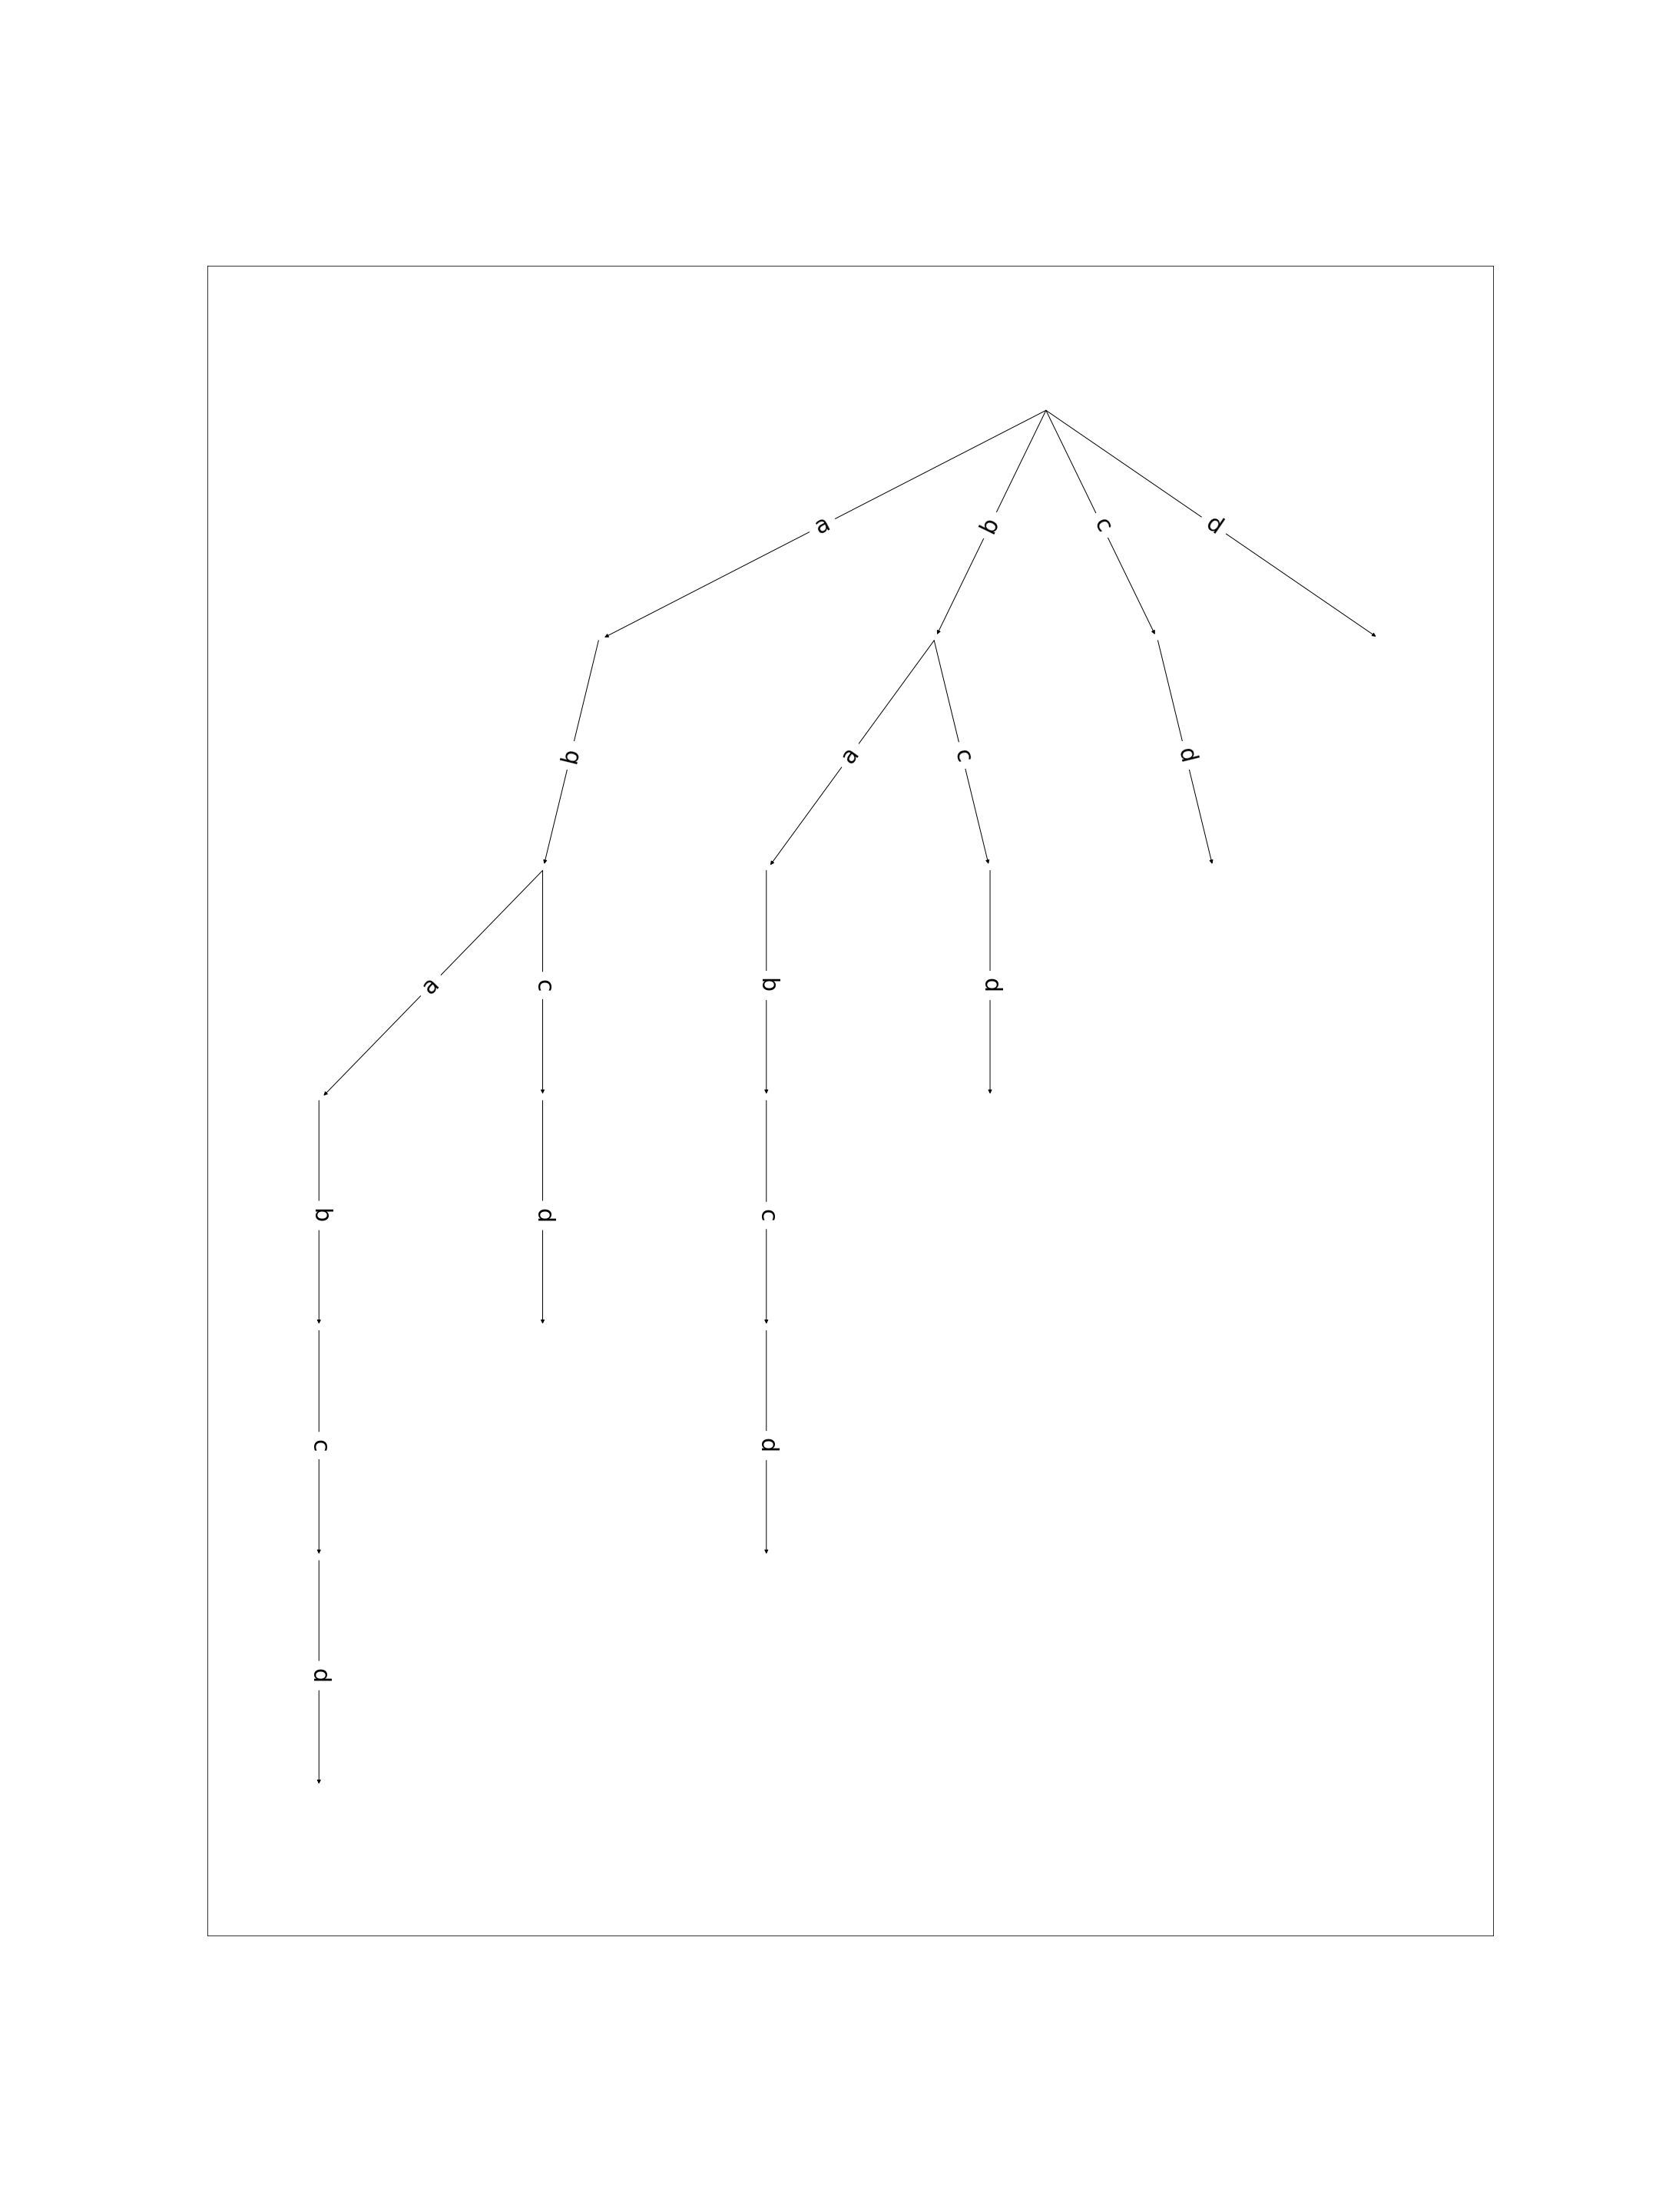
\includegraphics[width = \textwidth]{trie_example.png}
	\caption{Trie dla tekstu "ababcd"}
	\label{}
	\end{figure}
	
	\begin{figure}[htp]
	\centering
	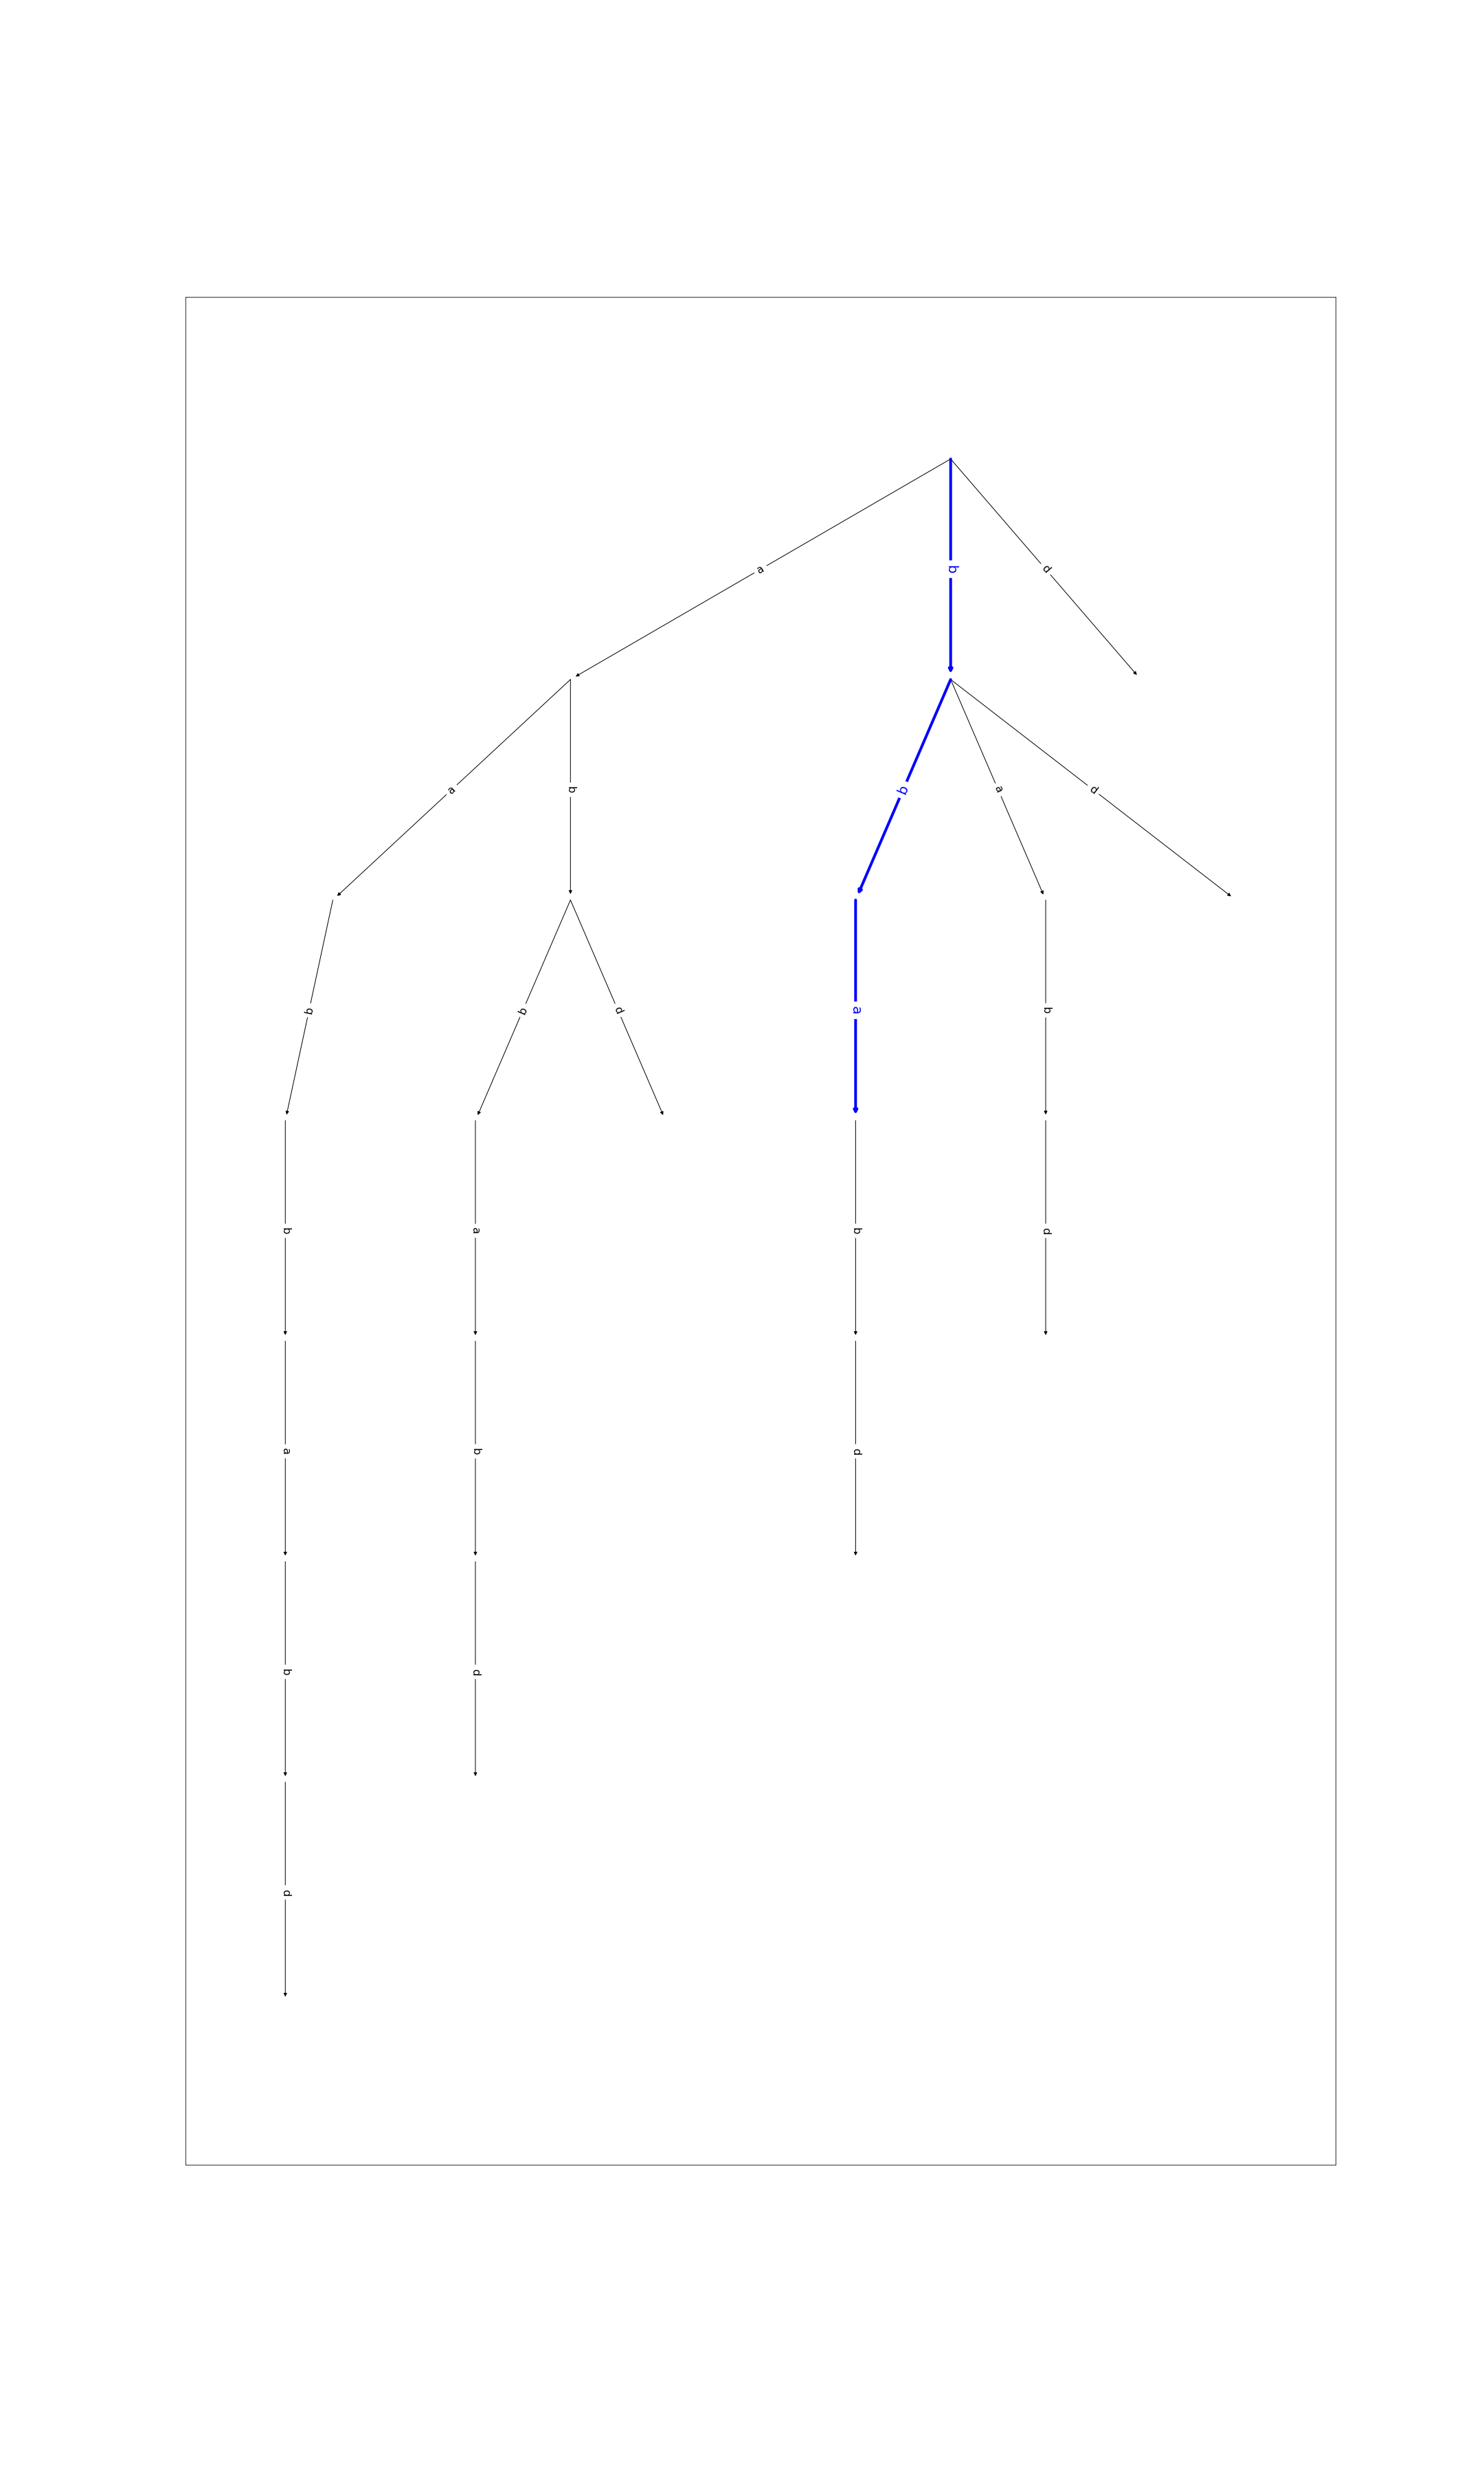
\includegraphics[width = \textwidth]{trie_text_example.png}
	\caption{Znalezione podsłowo "bba" w trie dla tekstu "aabbabd"}
	\label{}
	\end{figure}
	
	\begin{figure}[htp]
	\centering
	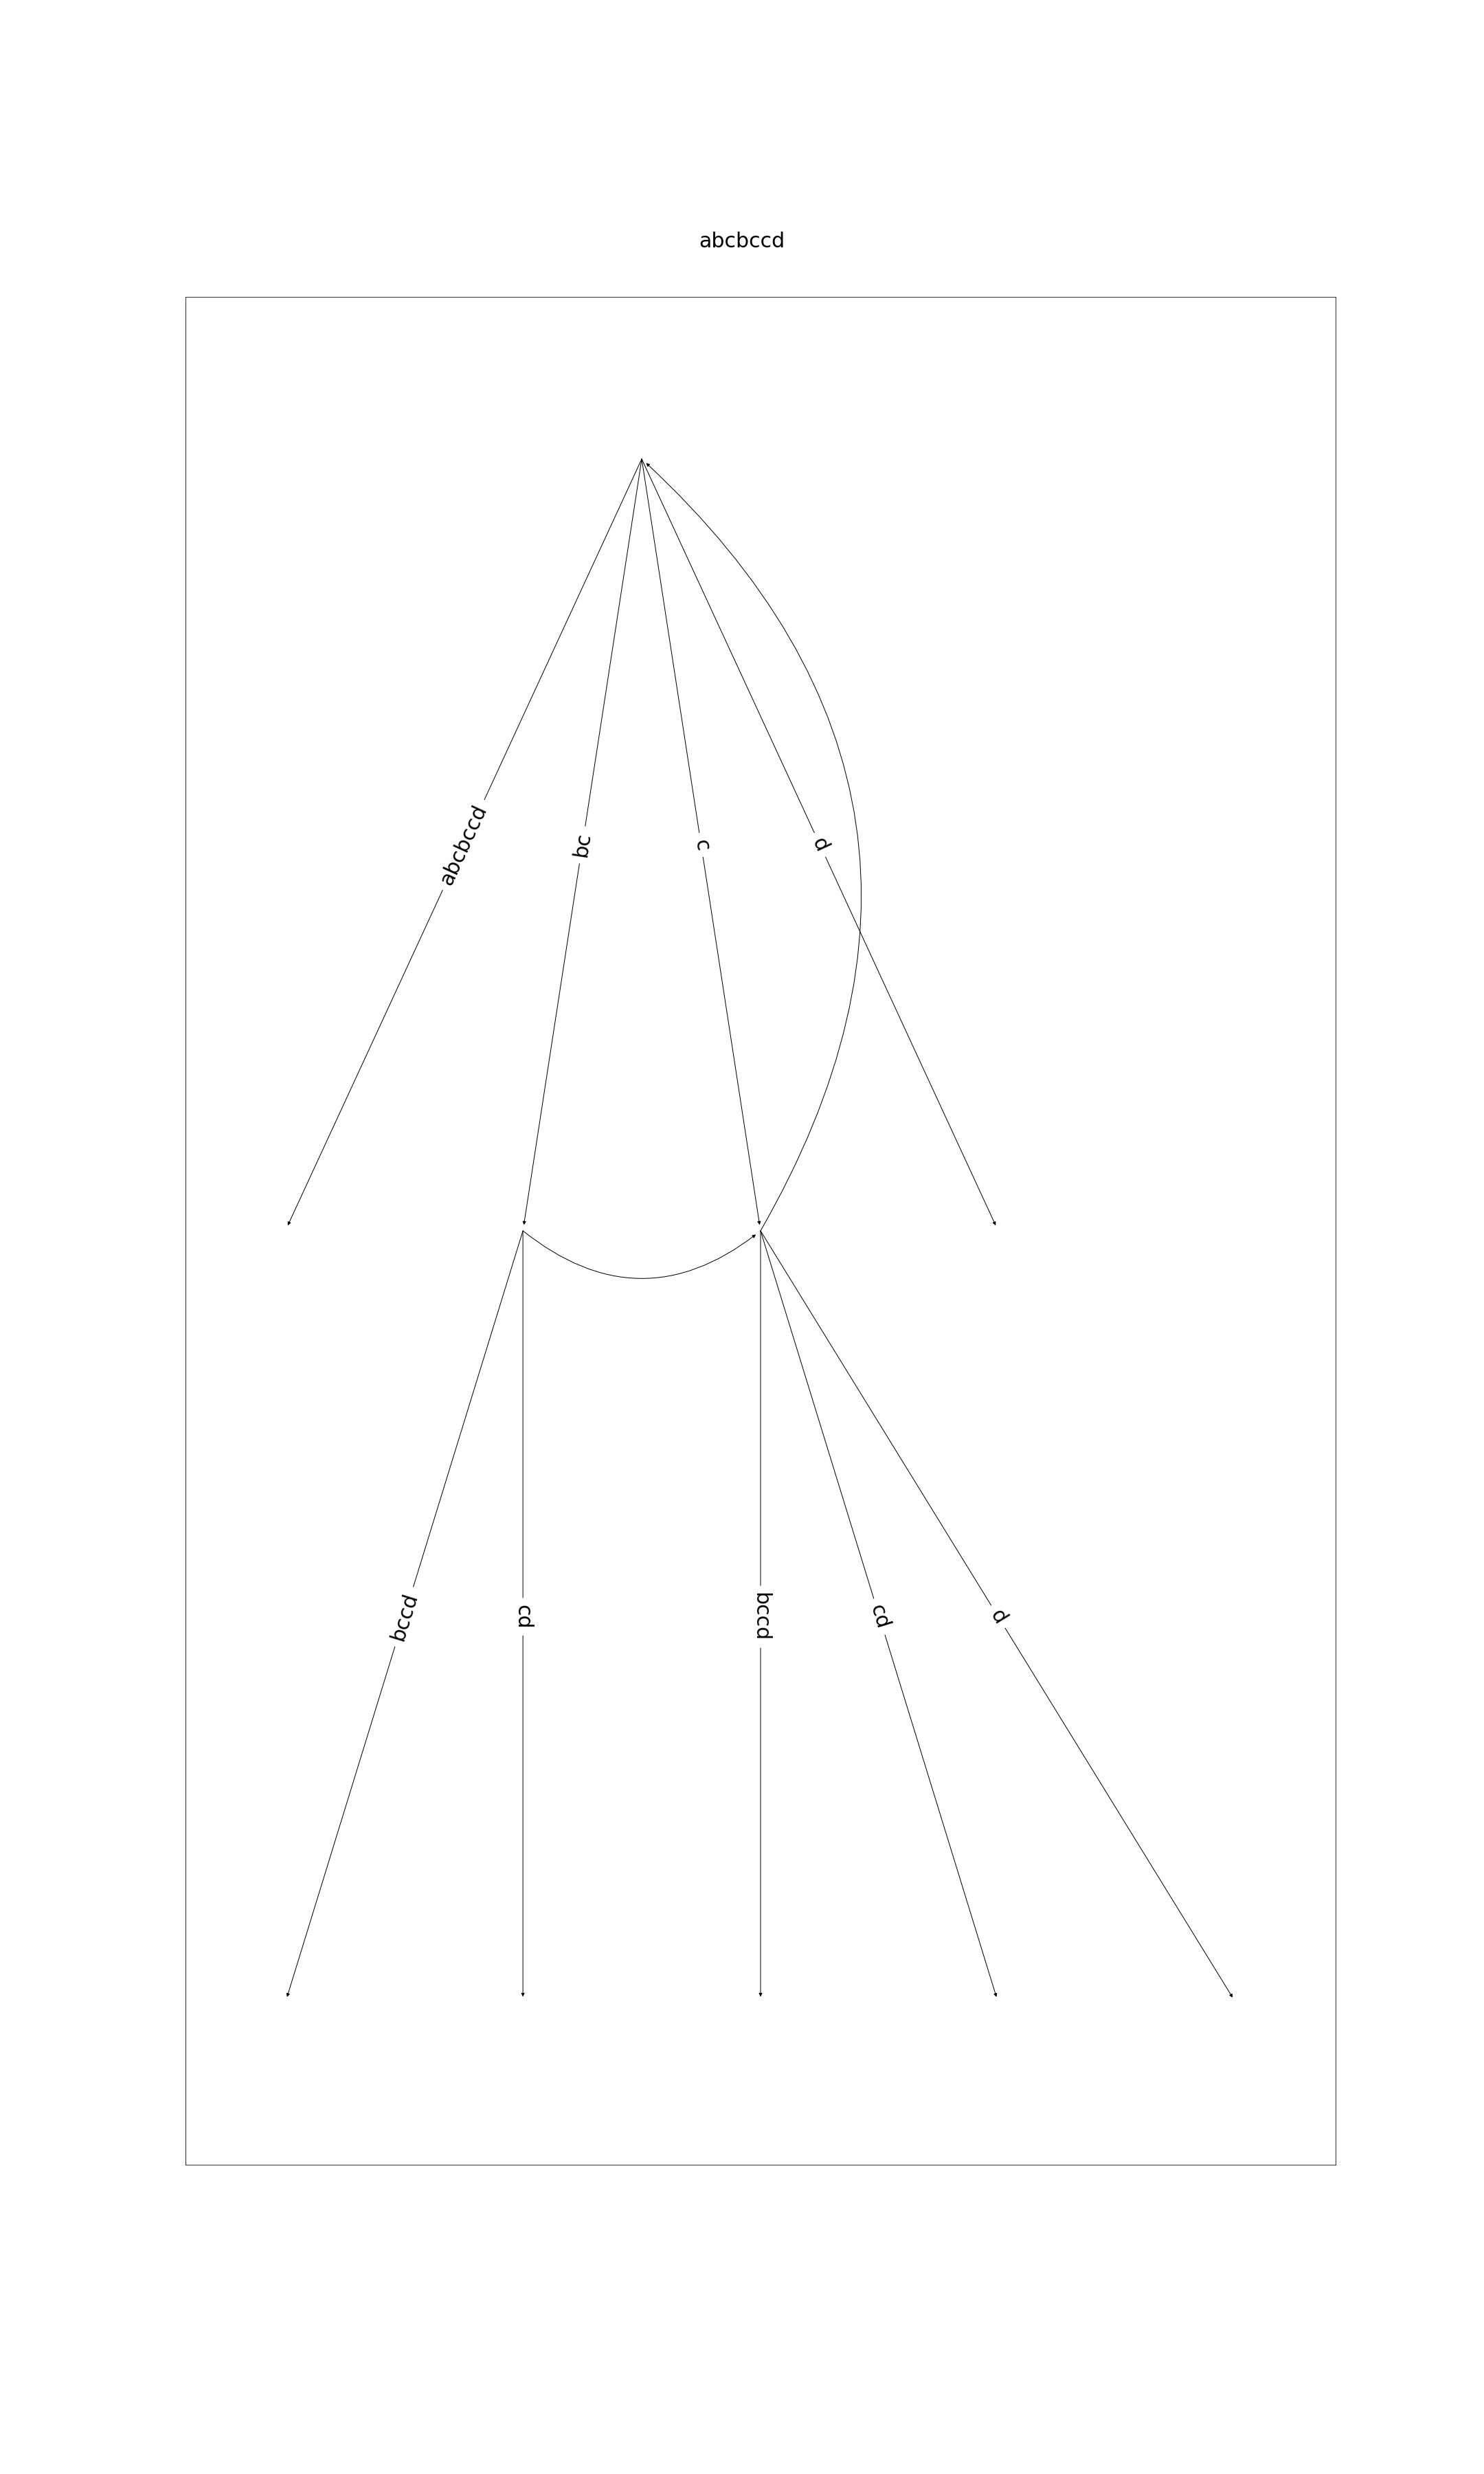
\includegraphics[scale=0.18]{suff_example.png}
	\caption{Drzewo sufiksów dla tekstu "abcbccd" zbudowane przy pomocy algorytmu McCreighta (krawędzie w kształcie łuków pokazują linki stworzone w trakcie działania algorytmu)}
	\label{}
	\end{figure}
\end{document}